%-*- coding:UTF-8 -*-
% 算法导论-第12章 二叉搜索树.tex
\documentclass[UTF8]{ctexart}
\usepackage{geometry}
\usepackage{enumerate}
\usepackage{amsmath}
\usepackage{listings} %插入代码
\usepackage{xcolor} %代码高亮
\usepackage{diagbox}
\usepackage{tabularx}
\usepackage{graphicx}
\usepackage{caption}
\usepackage{subcaption}
\usepackage{float}

% Some setup
\pagestyle{plain}
\geometry{a4paper, top=2cm, bottom=2cm, left=2cm, right=2cm}
\CTEXsetup[format={\raggedright\bfseries\Large}]{section}
\lstset{numbers=left, %设置行号位置
        numberstyle=\small, %设置行号大小
        keywordstyle=\color{blue}, %设置关键字颜色
        commentstyle=\color{purple}, %设置注释颜色
        %frame=single, %设置边框格式
        escapeinside=``, %逃逸字符(1左面的键),用于显示中文
        breaklines, %自动折行
        extendedchars=false, %解决代码跨页时,章节标题,页眉等汉字不显示的问题
        %xleftmargin=2em,xrightmargin=2em, aboveskip=1em, %设置边距
        tabsize=4, %设置tab空格数
        showspaces=false %不显示空格
       }

% About math
\newcommand{\rmnum}[1]{\romannumeral #1}

\begin{document}

\title{\Huge算法导论习题\\}
\vspace{2cm}
\author{\Large曾宇祥\\SY1406122}
\date{}
\maketitle

%\newpage
\section*{第12章\quad二叉搜索树}
\begin{enumerate}
    \item 12.1-5 \\
    解:\\
        首先考虑提示,基于比较的排序模型中,完成n个元素的排序最坏情况下需要$\Omega(nlgn)$
		的时间复杂度。需证明基于比较的算法构建二叉搜索树的最坏情况也为$\Omega(nlgn)$。\\
		显然,考虑利用$\Omega(nlgn)$的时间进行预排序构建有序数组,然后不断二分构建二叉树。
		此时构建的二叉树近似平衡,因此树高为$lgn$,因此建树的时间负责度为$\Omega(nlgn)$。\\
	
	\item 12.2-5 \\
	证明:\\
		显然用反证法证明该题目更为容易。假设$\forall p \in set(Nodes), p has two children.$,
		假设p的后继节点$p_0$且$p_0->left = q$, 则中序遍历该树(或子树)时q一定出现在$p_0$前,\\
		故p的后继节点至少不是$p_0$,因此可知假设错误。从而后继节点没左孩子的证。同理,前驱节点
		没右孩子使用反证法可证。

	\item 12.2-6 \\
	证明:\\
		题目的结论非常显然,使用反证法证明。不妨先假设y不是x的最顶层祖先,又因为y是x的后继,
		因此y一定不能出现在x的左子树,那么y只能出现在x的右子树,这与已知条件x的右子树为空矛盾。\\
		故可知y一定是x的祖先,因此,y的左孩子为x或者x的祖先(或者祖先的祖先...)。
		故y的左孩子一定是x的祖先。
		
	\item 12.2-7 \\
	证明:\\
		这题目的算法时间复杂度很显然,考虑Minimum过程主要遍历的是树的左子树,而每当当前结点的右子树
		不为空时,Successor过程再次调用Minimum过程遍历该结点右孩子的左子树,否则右结点为空,向上回溯
		找到该结点的后继结点,因此全部结点被遍历2次,故时间复杂度为$theta(n)$.
		
	\item 12.2-8 \\
	证明:\\
		采用第二数学归纳法证明:
		当$k=1$时,根据Successor过程可知若当前结点右子树不为空,则调用Minimum过程,因此,此时时间复杂度
		为$O(n+1)$, 故此时满足结论;\\
		当$k>1$时,不妨假设$k<k_0$是,结论成立,仅需证明当$k=k_0$时结论同样成立,因此,
		$T(n) = O(k_0-1+h) + T(1)$, 而$T(1) = O(1+h)$, 则$T(n) = O(k+h+h) < 2(k+h) = O(k+n)$.	\\
		故原结论得证。
	
	\item 12.2-9 \\
	证明:\\
		采用反证法证明。\\
		不妨假设y.key不是T树中大于x.key的最小关键字,或者也不是小于x.key的最大关键字。
		即存在结点p使得p.key是T树中大于x.key的最小关键字,且p不等于x
		  存在结点q使得p.key是T树中小于x.key的最大关键字,且q不等于x。\\
		因为x为叶子结点,因此当p为T树中大于x.key的最小关键字,p只可能等于x。因此假设1错误,
		同理,q也只能等于x。因此假设2错误。\\
		故原结论成立。
		
	\item 12.3-2 \\
	证明:\\
		这个题目很无聊,设想插入一个元素x的插入过程其实就是一个搜索x的最恰当插入位置的过程,
		从而当真正查找元素x时,走过原来的路径,再查找元素x即可以从查找过程返回。\\
		因此,查找检查的结点数目是插入检查的结点数目加1。
	
	\item 12.3-3 \\
	解:\\
		最坏情况,就是元素有序,$T(n) = 1+2+\cdots+n = O(n^2)$,
		最好情况就是元素平衡,此时时间复杂度为$O(nlgn)$。
		
	\item 12.3-4 \\
	解: \\
		不可交换。\\
		\begin{figure}[H]
		\centering
        \caption{12.3两种删除方式的反例示意图}
		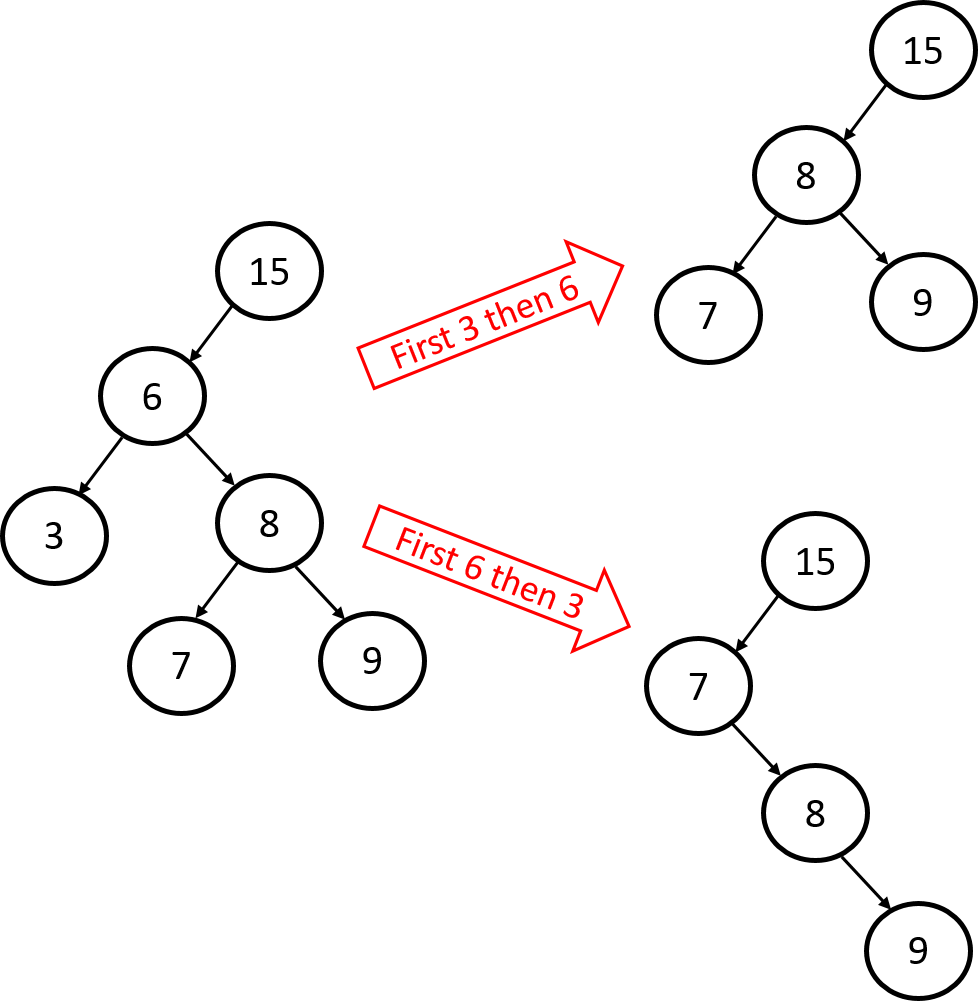
\includegraphics[scale=0.65]{1203_4.png}
		\end{figure}
	
	\item 12.3-5 \\
	解:\\
		中文的算法导论这个题目翻译错了,英文的题目的意识是使用x.succ属性代替s.p属性。
		如提示所示,就是利用后继的属性重新实现插入、删除、查找函数。\\
		求结点p的父节点的思路是先求得p所在子树的最大值,该值所在结点的后继就是p的父节点。
		其余操作均需要利用后继的性质。以插入为例。\\
		\begin{lstlisting}[language=]
			void Tree_Insert(Tree_t *t, Node_t *z) {
				Node_t *y = NULL;
				Node_t *x = t->root;
				while (x != NULL) {
					y = x;
					if (z->key < x->key)
						x = x->l;
					else
						x = x->r;
				}
				if (y == NULL) {
					t->root = z;	// tree t was empty
					z->succ = NULL;
				} else if (z->key < y->key) {
					Node_t *p = ParentOf(y);
					z.succ = y;
					p.succ = z;
				} else {
					z->succ = y->succ
					y->succ = z;
				}
			}
        \end{lstlisting}
		
\end{enumerate}


\end{document}

